\chapter{The prepare and measure scenario}
\label{chap:pam}

    The prepare and measure (PM) scenario is one of the simplest and most fundamental examples of correlation scenarios. In it, a preparation apparatus produces and then sends a physical system, over a communication channel, to a measurement device which reads out information from the received state. Wherefore, it is an adequate setting in which to investigate two of the most fundamental building blocks of physical theories: states and measurements. Prepare and measure scenarios are also the simplest correlation scenarios that presume communication, and, as such, should become an indispensable ingredient in quantum networks \cite{bowles_pamnetworks_2015,poderini_pamcriteria_2020}. As with other correlation scenarios, quantum behaviors in the PM scenario can be exploited to build informational protocols that show advantage over their classical counterparts (sec. \ref{sec:communication-protocols}). On a more fundamental aspect, they are at the core of proposed informational principles to quantum theory \cite{pawlowski_infocausality_2009,pawlowski_infocausalityreview_2011}, and of quantum ontologies \cite{spekkens_2005_contextuality}.

    Differently from the more widely studied Bell nonlocality and EPR steering scenarios, a quantum prepare and measure experiment may behave nonclassically even in the absence of entanglement. Quantum behaviors in PM scenarios must then rely on other strictly quantum features, such as measurement incompatibility \cite{carmeli_racsincompatibility_2020} and non-orthogonality of states \cite{brunner_dimension_2013}, but the exact relations are still unknown. Other than quantum communication, a second resource that also leads to drastically different behaviors is whether the preparation and measurement devices are independent or not. There are, in general, three possible cases; namely, full independence, shared randomness and entanglement assistance. Together with either classical or quantum communication, this will lead to six nonequivalent prepare and measure configurations.

    In chapters \ref{chap:pam-classical} and \ref{chap:pam-quantum}, novel results regarding some of these settings will be presented. To build towards that end, we now discuss these many different instances of preparation and measurement devices, and show how this scenario can be seen as a physical implementation of two paramountly important communication protocols.

    %%%%%%%%%%%%%%%%%%%%%%%%%%%%%%%%%%%%%%%%%%%%%%%%
    \section{Prepare and measure behaviors}

        The simplest prepare and measure setup consists of two black-boxes. One is the preparation device P, handled by Alice, and the other the measurement device M, handled by Bob. Nothing about the inner workings of these devices is assumed \emph{a priori}, except that P prepares and communicates a physical system to M, which extracts information from the received preparation by measuring it.
    
        Alice is allowed to interact with her device through a classical input $x \in \mathcal{X} \equiv \natrange{X} \equiv [X]$. Her choice may weight on the probability $\condprob{m}{x}$ with which a state, labeled by $m$, from a set $\mathcal{S}$, is prepared. Here, $\mathcal{S}$ represents the set of possible preparations. Alice's choice of $x$ can be more intuitively understood as the message she wants to encode and communicate to Bob, and an $m \in \mathcal{S}$ as the carrier of that information. On his end, Bob can choose a configuration $y \in \mathcal{Y} \equiv [Y]$ for the measurement device, which will thence output $b \in \mathcal{B} \equiv [B]$ with probability $\condprob{b}{m,y}$. This reflects the fact that the outcome of the experiment may be influenced by both the received message and Bob's choice of measurement (fig. \ref{fig:pam-scenario}). More intuitively, $Y$ limits how many choices of decoding procedures can be used by Bob to try and recover Alice's message $x$.

		\begin{figure}
			%
			\begin{minipage}[c]{0.41\textwidth}
				\centering
				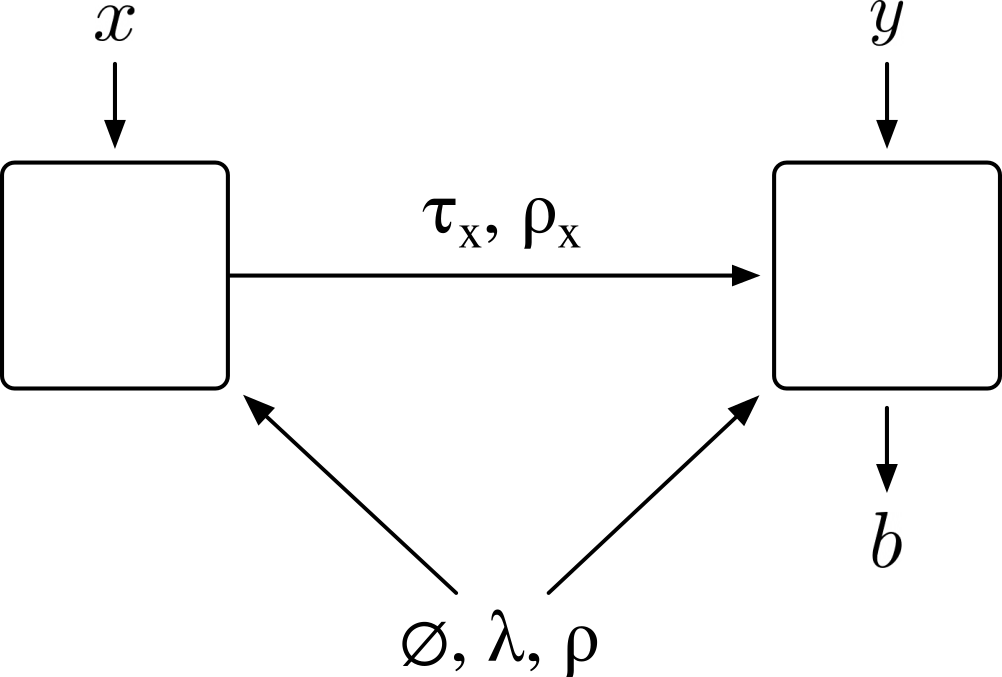
\includegraphics[width=.8\columnwidth]{pam_scenario.png}
			\end{minipage}
			%
			\begin{minipage}[c]{0.58\textwidth}
				\caption{Prepare and measure scenarios. The measurement box, upon receiving an input $x$, prepares either a classical, $\tau_x$, or quantum $\rho_x$, state to the measurement device. In turn, given a choice $y$ of measurement, an output $b$ is observed. From their causal past, the devices may be independent ($\emptyset$), share classical randomness ($\lambda$), or even quantum correlations ($\rho$).}	
				\label{fig:pam-scenario}
			\end{minipage}
			%
		\end{figure}

        A last, indispensable condition is that neither Alice nor Bob know what happens in each other's labs. In other words, she must have no knowledge of $y$, as this is a choice made in her causal future, and he cannot know what was her choice $x$ of preparation, as this trivializes communication. Taken together, these constraints amount to saying that all exchanges of information between them are mediated by the message $m$. Given that our intention is to study how this communication influence the observed statistics, this is clearly a natural assumption.
        
        A \emph{round} is a single run of the protocol described above. After many such rounds, Alice and Bob are allowed to share their data with each other, and together they can build the \emph{behavior} $\mathbf{p} = \{ \condprob{b}{x,y} \}_{b,x,y}$ of their devices. This behavior characterizes the prepare and measure \emph{experiment}. Naturally, each $\condprob{b}{x,y} \geq 0$ and $\sum_b \condprob{b}{x,y} = 1, \,\forall x,y$, or, equivalently, $\mathbf{p}$ is a collection of conditional probability distributions, one for any fixed choice of a pair $(x,y)$.
        
        We now arrive at the central question of (semi)device-independent quantum information: if all we have is the behavior $\mathbf{p}$, with no (or restricted) access to the internal workings of the devices, can we still certify some property about the states, measurements, or other quantities of interest? For instance, could we, by only observing $\mathbf{p}$, affirm that P prepares quantum --- as opposed to classical ---, states? Or that M applies nonprojective measurements? In many cases, the answer, surprisingly, is \emph{yes}.
    
        %%%%%%%%%%%%%%%%%%%%%%%%%%%%%%%%%%%%%%%%%%%%%
        \subsection{Classical preparations}
        \label{sec:classical-behaviors}

            Quantum preparations may behave distinctly from classical preparations, and knowing how to tell them apart is of the essence in developing quantum communication protocols. An important open question regards the exact properties that allow some sets of preparations and measurements to behave nonclassically. In chapter \ref{chap:pam-classical}, we will discuss the problem of classical simulatability of quantum behaviors in reasonable generality, and prove that measurement incompatibility --- a candidate for the origin of nonclassicality in PM scenarios --- is not sufficient. To make that discussion precise, we must begin by defining what it is that we will call classically-simulatable behaviors or, for shortness, \emph{classical behaviors}.
        
            Starting from the paradigmatic prepare and measure scenario, let us further impose that $\mathcal{S}$, the set of possible preparations, contains only \emph{classical states} (dits). Naturally, as this is a communication scenario, the dimension $\abs{\mathcal{S}}$ of the classical system used for encoding the states must be bounded, otherwise communication becomes trivial (i.e., Alice can perfectly encode her message $x$, and Bob can perfectly recover it).
            
            Our first aim is to investigate the set of behaviors that can be achieved when communicating $d$-dimensional classical systems, or rather, when  $\mathcal{S} = \posrange{d-1}$. They will, in general, also depend on $X$ (the size of Alice's input alphabet) and $Y$ (the number of choices for Bob's measurement). Letting this set of behaviors be $\mathcal{C}_{d,X,Y}$, our previous discussion implies that
            %
            \begin{equation}
                \mathbf{p} \in \mathcal{C}_{d,B,X,Y} \quad\Longleftrightarrow \quad \condprob{b}{x,y} = \sum_{m \in \mathcal{S}} \condprob{m}{x} \condprob{b}{m,y} \quad\forall b,x,y .
                \label{eq:pam-classical-independent}
            \end{equation}
            %
            Essentially, then, $\mathcal{C}_{d,B,X,Y}$ contains all behaviors that may occur when (i) the devices are \emph{uncorrelated}, (ii) the preparations are classical and (iii) with dimension at most $d$, (iv) Alice has $X$ preparation choices, and (v) Bob picks one out of $Y$ measurement settings with (vi) $B$ outcomes each. If the parameters are clear by the context, we simplify the notation by omitting subscripts.
            
            Briefly detouring, it is interesting to notice that model~\eqref{eq:pam-classical-independent} is much in the spirit of ontological models \cite{spekkens_2005_contextuality,harrigan_2008_ontological,galvao_2009_economical}. To see that, consider $\mathcal{S}$ as a finite, dimension-bounded ontic state space, and $x$ as the preparation procedure. Then, $\condprob{m}{x}$ models our epistemic state. Similarly, if we take $y$ as a choice of measurement procedure, we may interpret $\condprob{b}{m,y}$ as the indicator function. In this way, any theory that only produces behaviors $\mathbf{p} \in \mathcal{C}_{d,B,X,Y}$ admits a dimension-bounded ontological model.
            
            Conditions (iii)--(vi) above are natural for any communication scenario, but the case is different for (i) and (ii). While in many situations, such as when we have some trust on our devices, (i) is justifiable, it is not always safe to assume that the devices are uncorrelated. The worst-case scenario for classical variables is when P and M can share an unbounded amount of pre-established \emph{classical correlations}. Such correlations must reside in the causal past of the experiment (fig. \ref{fig:pam-dag}), but even so, they can be used to achieve better performance in several communication protocols implemented in the PM scenario \cite{de_vicente_bound_2019}, and lead to quite different geometrical structures \cite{de_vicente_shared_2017,dallarno_robustness_2012}. Without knowledge on what correlations the devices share, the best we can do is to call it $\lambda$ and say that $\pi$ is some probability distribution over this random variable. As both devices can fully access $\lambda \in \Lambda$,
            %
            \begin{equation}
                \mathbf{p} \in \mathcal{C}_{d,B,X,Y}^\lambda \quad\Longleftrightarrow \quad \condprob{b}{x,y} = \int_{\Lambda} \sum_{m \in \mathcal{S}} \pi(\lambda) \condprob{m}{x,\lambda} \condprob{b}{m,y,\lambda} d\lambda \quad\forall b,x,y .
                \label{eq:pam-classical-sr}
            \end{equation}
            %
            Here, $\mathcal{C}_{d,B,X,Y}^\lambda$ is the set of behaviors we get from $\mathcal{C}_{d,B,X,Y}$ by allowing for classical correlations, or \emph{shared randomness} (SR). As $\pi(\lambda) \geq 0$ and $\sum_\lambda \pi(\lambda) = 1$, eq.~\eqref{eq:pam-classical-sr} is actually telling us that $\mathcal{C}_{d,B,X,Y}^\lambda = \conv{\mathcal{C}_{d,B,X,Y}}$ (eq.~\eqref{eq:convex-hull}). Because $\mathcal{C}_{d,B,X,Y}^\lambda \subseteq \mathcal{C}_{d,B,X,Y}$ and $\mathcal{C}_{d,B,X,Y}$ is not convex, it holds that $\mathcal{C}_{d,B,X,Y} \subset \mathcal{C}^\lambda_{d,B,X,Y}$. More than that, a slight variation on Fine's theorem \cite{fine_hidden_1982} (or sec. 2.3 of \cite{scarani_bell_2019}, for a more pedagogical discussion) can show that the set $\mathcal{C}_{d,B,X,Y}$ has a finite amount of extremal points, called deterministic strategies \cite{gallego_pam_2010,de_vicente_bound_2019}. They are the points given by eq.~\eqref{eq:pam-classical-sr} when the response functions are deterministic, i.e., when $\condprob{m}{x} = \delta_{m,f(x,\lambda)}$ and $ \condprob{b}{m,y} = \delta_{b,g(m,y,\lambda)}$, for some functions $f : \mathcal{X} \rightarrow \posrange{d-1}$ and $g : \posrange{d-1} \times \mathcal{Y} \rightarrow \mathcal{B}$ that are made precise in the aforementioned references. Interpreting $\mathcal{C}_{d,B,X,Y}^\lambda$ as a convex hull of finitely many points, this proves that $\mathcal{C}_{d,B,X,Y}^\lambda$ is a polytope. Recalling the discussion in sec. \ref{sec:convexity}, we emphasize that $\mathcal{C}_{d,B,X,Y}^\lambda$ can thus be described by an intersection of half-spaces, which are given by the linear inequalities defining its facets. This description will turn out to be especially useful along chap. \ref{chap:pam-classical}, in which we will get back to this topic and work out an example that should clarify this discussion.

			\begin{figure}
			%
				\begin{minipage}[c]{0.31\textwidth}
					\centering
					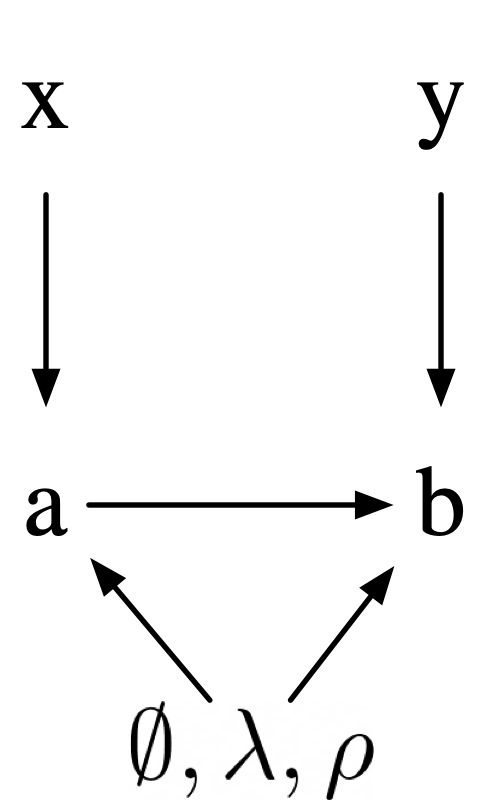
\includegraphics[width=.5\columnwidth]{pam-dag.png}
				\end{minipage}
				%
				\begin{minipage}[c]{0.68\textwidth}
					\caption{Causal structure of a prepare and measure experiment. Choice $x$ of preparation can only directly influence the message $m$, which can be encoded in a classical or quantum system. Communicating $m$ effectively screens-off the choice of $x$, unless the measurement device can perfectly recover it. Observable $b$ is influenced by the received message $m$ and the choice $y$ of measurement, which can be seen as a decoding function. Both $m$ and $b$ can be further classically or quantumly correlated by some variable in the causal past of the experiment.}	
					\label{fig:pam-dag}
				\end{minipage}
			\end{figure}
            
            For an example of the usefulness in understanding these sets, notice that for some fixed $X$ and $Y$, and some $d^\prime > d$, we have the proper inclusion $\mathcal{C}_{d} \subset \mathcal{C}_{d^\prime}$, which implies the same for the SR case. Ultimately, this means that larger dimensional communication can carry more information. Now suppose that $W_d$ is a linear functional defining some facet of $\mathcal{C}_{d}^\lambda$ which is not a facet of $\mathcal{C}_{d^\prime}^\lambda$ (at least one such $W_d$ must exist, since $\mathcal{C}_{d}^\lambda \subset \mathcal{C}_{d^\prime}^\lambda$) and that, for any behavior $\mathbf{p} \in \mathcal{C}_d^\lambda$, we have a bound $W_d \cdot \mathbf{p} \leq C_d$. Because $W_d$ does not define a facet of $\mathcal{C}_{d^\prime}^\lambda$, there is some $\mathbf{p}^\prime \in \mathcal{C}_{d^\prime}^\lambda$ such that $W_d \cdot \mathbf{p}^\prime > C_d$. Hence, if we are given preparation and measurement boxes which are guaranteed to prepare only classical systems, and we observe some behavior that, like $\mathbf{p}^\prime$, violates the bound on $W_d$, we can certify that Alice's device is preparing classical states of dimension at least $d+1$.
            
            In disguise, I have exemplified what is called a (dimension) witness: any functional and bound that, (i) for some set of behaviors is never violated, but that (ii) can be violated by at least one behavior of some other set, is said to \emph{witness} some property. In our case, we are witnessing dimension in a semi-device-independent fashion, as we have assumed the preparations are classical. Lastly, notice that the facets defining any $\mathcal{C}_d^\lambda$ polytope are, by definition, dimension witnesses. Furthermore, they are \emph{tight} witnesses, something which not all witnesses must be.
            
            For completeness, we note it is also possible to define $\mathcal{C}_{d,B,X,Y}^{\rho}$ sets, where the preparations remain classical, but the devices can be correlated through a shared quantum state $\rho$ \cite{tavakoli_eapam_2021,poderini_pamcriteria_2020}. When $\rho$ is an entangled state, this can lead to interesting behaviors associated with advantages in communication protocols \cite{pawlowski_earacs_2010}. Generally, $\mathcal{C}^\lambda_{d,B,X,Y} \subseteq \mathcal{C}^\rho_{d,B,X,Y}$, but the results in \cite{pawlowski_earacs_2010} imply that strict inclusion holds for at least some cases.

    
        %%%%%%%%%%%%%%%%%%%%%%%%%%%%%%%%%%%%%%%%%%%%%%
        \subsection{Quantum preparations}
        \label{sec:quantum-behaviors}

            Generalizing our discussion, let us also remove the assumption of classical preparations. In that case, $\mathcal{S}$ will be a finite subset of $\mathcal{D}(\hilb)$, and $y$ a choice of a quantum measurement. Employing Born's rule, the behaviors may be rewritten as $\mathbf{p} = \{ \tr{\rho_x E_{b \vert y}} \}_{b,x,y}$. Here, all $\rho_x \in \mathcal{S}$, and $\{ E_{b \mid y} \}_b$ is a POVM for each $y$. For the dimension bound, let $\text{dim}(\mathcal{S}) = \text{dim} \sum_{\rho_x \in \mathcal{S}}\text{supp}\left( \rho_x \right)$ be the smallest Hilbert space dimension needed to represent all density operators in $\mathcal{S}$. Then, in direct analogy to the classical behaviors sets, for any fixed $X$ and $Y$, we define $\mathcal{Q}_{d,B,X,Y}$ as the set of behaviors arising from quantum communication with uncorrelated devices.
            
            Allowing for shared randomness introduces a slight change in the elements of the behaviors. Using the same notation as before, they turn into
            %
            $$
                \condprob{b}{x,y} =  \int_\Lambda \pi(\lambda) \tr{\rho_x^\lambda E_{b \vert y}^\lambda} ,
            $$
			and $\mathcal{Q}^\lambda_{d,B,X,Y}$ would be the sets of such behaviors. Regarding set inclusions, clearly $\mathcal{Q}_{d,B,X,Y} \subseteq \mathcal{Q}^\lambda_{d,B,X,Y}$, but results in \cite{ambainis_srqracs_2009} prove there are instances where $\mathcal{Q}_{d,B,X,Y} \subset \mathcal{Q}^\lambda_{d,B,X,Y}$.
            %
			% \review{If it weren't for the $\lambda$'s in the preparations and measurements, then $\mathcal{Q}^\lambda$ would be $\conv{\mathcal{Q}}$. But, as $\mathcal{Q}$ is already convex, this would imply that they are equal. However, the $\lambda$'s inside the trace may make a difference. Do they? Could be nice to cite some ref. about this but I don't remember any.}
            
            Lastly, and most importantly for chap. \ref{chap:pam-quantum}, Alice and Bob may share a quantum system $\rho \in \hilb_A \otimes \hilb_B$ and exploit it as a resource to improve their quantum communication. That is what we call an \emph{entanglement-assisted} scenario. Most generally, Alice can use her share of $\rho$ as an aid in her encoding of $x$, and the way to do it is by applying a local CPTP map $\Lambda_x$ to her share of $\rho$. As we must bound the communication to $d$-dimensional systems, $\Lambda_x : \mathcal{L}(\hilb_A) \rightarrow \mathcal{L}(\hilbd{d})$, where $\hilbd{d} \simeq \mathbb{C}^d$. This system in $\hilbd{d}$ is then transmitted to Bob, who will afterwards hold $\rho_x = \left( \Lambda_x \otimes \id_B \right) \rho$. His measurements' effects act on $\hilbd{d} \otimes \hilb_B$. Behaviors compatible with experiments implementing this procedure are in the sets $\mathcal{Q}^\rho_{d,B,X,Y}$, and dense coding (sec. \ref{sec:dense-coding}) provides examples where $\mathcal{Q}^\lambda_{d,B,X,Y} \subset \mathcal{Q}^\rho_{d,B,X,Y}$. Sometimes, it is a reasonable assumption to make $\hilb_A \simeq \hilbd{d}$ (see sec. \ref{sec:dense-coding} and chap. \ref{chap:pam-quantum}). Bear in mind, though, that it can lead to some loss of generality: recently, Tavakoli et al. \cite{tavakoli_eapam_2021} considered a qubit communication protocol where $4$-dimensional entanglement shows advantage over having only a $2$-dimensional entangled resource. To the best of my knowledge, those, together with Moreno et al.'s (\cite{moreno_pamdense_2021} and chap. \ref{chap:pam-quantum}), were the first results considering this most general quantum communication scenario.
            
            As a side note, although I have presented entanglement-assisted quantum communication scenarios as the most general kind of PM scenario, there are still further possible generalizations if we allow Alice's and/or Bob's inputs $x$ and $y$ to also be quantum variables \cite{guerini_distributed_2019}. These are interesting and little explored scenarios, but dealing with them is out of our scope.
            
            Clearly, any of the sets $\mathcal{Q}$, $\mathcal{Q}^\lambda$ and $\mathcal{Q}^\rho$ is contained in their respective larger-dimensional counterparts. Thence, the same observations made before make it possible to also derive \emph{quantum} dimension witnesses \cite{gallego_pam_2010}. Whereas witnessing dimension for classical or quantum preparations is already of practical and fundamental interest, we ideally want to also distinguish between classical and strictly quantum behaviors. To that end, it is useful to recognize that all behaviors from a set of $d$-dimensional pair-wise commuting density operators can be reproduced by communicating classical systems of a dimension that need not be larger than $d$. More precisely, if $\mathcal{S}_C$ is a set of $d$-dimensional density operators such that $\left[ \rho_i, \rho_j \right] = 0, \,\forall \rho_i, \rho_j \in \mathcal{S}_C$, then they can be simultaneously diagonalized w.r.t. some orthonormal basis $\{ \ket{ e_i } \}_{i=1}^d$. There can be at most $X=d$ $d$-dimensional preparations with this property. Letting $\rho_x = \sum_i c_{i,x} \ketbra{e_i}{e_i}$, we get that $\tr{ E_{b \mid y} \rho_x } = \sum_i c_{i,x} \braopket{e_i}{E_{b \mid y}}{e_i}$. Operationally, this means that communicating the label $x$ (a classical variable with dimension $d \geq X$) is enough to reproduce all possible behaviors: upon getting $x$ and Bob's choice $y$, the measurement device samples $\ket{e_i}$ with probability $c_{i,x}$, measures it considering $y$, and after collecting asymptotically many results the parties recover the correct $\condprob{b}{x,y}$.  
            
            However, not all quantum states commute. For any fixed $B,X,Y$ and $d < X$, then, it holds that $\mathcal{C} \subset \mathcal{Q}$, and similarly for the quantum sets allowing for shared randomness and entanglement assistance. More than that, recall that $\mathcal{C}^\lambda = \conv{\mathcal{C}}$, i.e., $\mathcal{C}^\lambda$ is the \emph{smallest} convex set that contains $\mathcal{C}$ (sec. \ref{sec:convexity}). Jointly with the fact that $\mathcal{Q}$ is convex and $\mathcal{C} \subset \mathcal{Q}$, we must have that $\mathcal{C}^\lambda \subseteq \mathcal{Q}$. Gallego et al. have further shown that actually $\mathcal{C}^\lambda \subset \mathcal{Q}$ \cite{gallego_pam_2010}, as illustrated in fig. \ref{fig:pam-behaviors}. Collecting the aforementioned set relationships, we find that, for fixed $B, X, Y$ and $d < X$, 
            %
			\begin{subequations}
            \begin{align}
                &\mathcal{C} \subset \mathcal{C}^\lambda \subset \mathcal{Q} \subseteq \mathcal{Q}^\lambda \subseteq \mathcal{Q}^\rho\, , \text{ and} \\
                %&\mathcal{C} \subset \mathcal{C}^\lambda \subset \mathcal{Q} \subseteq \mathcal{Q}^\lambda \subseteq \mathcal{Q}_d^\rho\, , \text{ and} \\
                &\mathcal{C} \subset \mathcal{C}^\lambda \subseteq \mathcal{C}^\rho \subseteq \mathcal{Q}^\rho\, .
            \end{align}
			\end{subequations}
            %
            Noticing that $\mathcal{C}^\lambda$ is the largest of the purely classical sets, and $\mathcal{Q}$ the smallest set of behaviors involving quantum variables, the relation $\mathcal{C}^\lambda \subset \mathcal{Q}$ shows we can build nonclassicality witnesses for the prepare and measure scenario. Although I would be surprised if not all relations above are proper inclusions, affirming that demands more careful consideration.

			\begin{figure}
				%
				\begin{minipage}[c]{0.43\textwidth}
					\centering
	                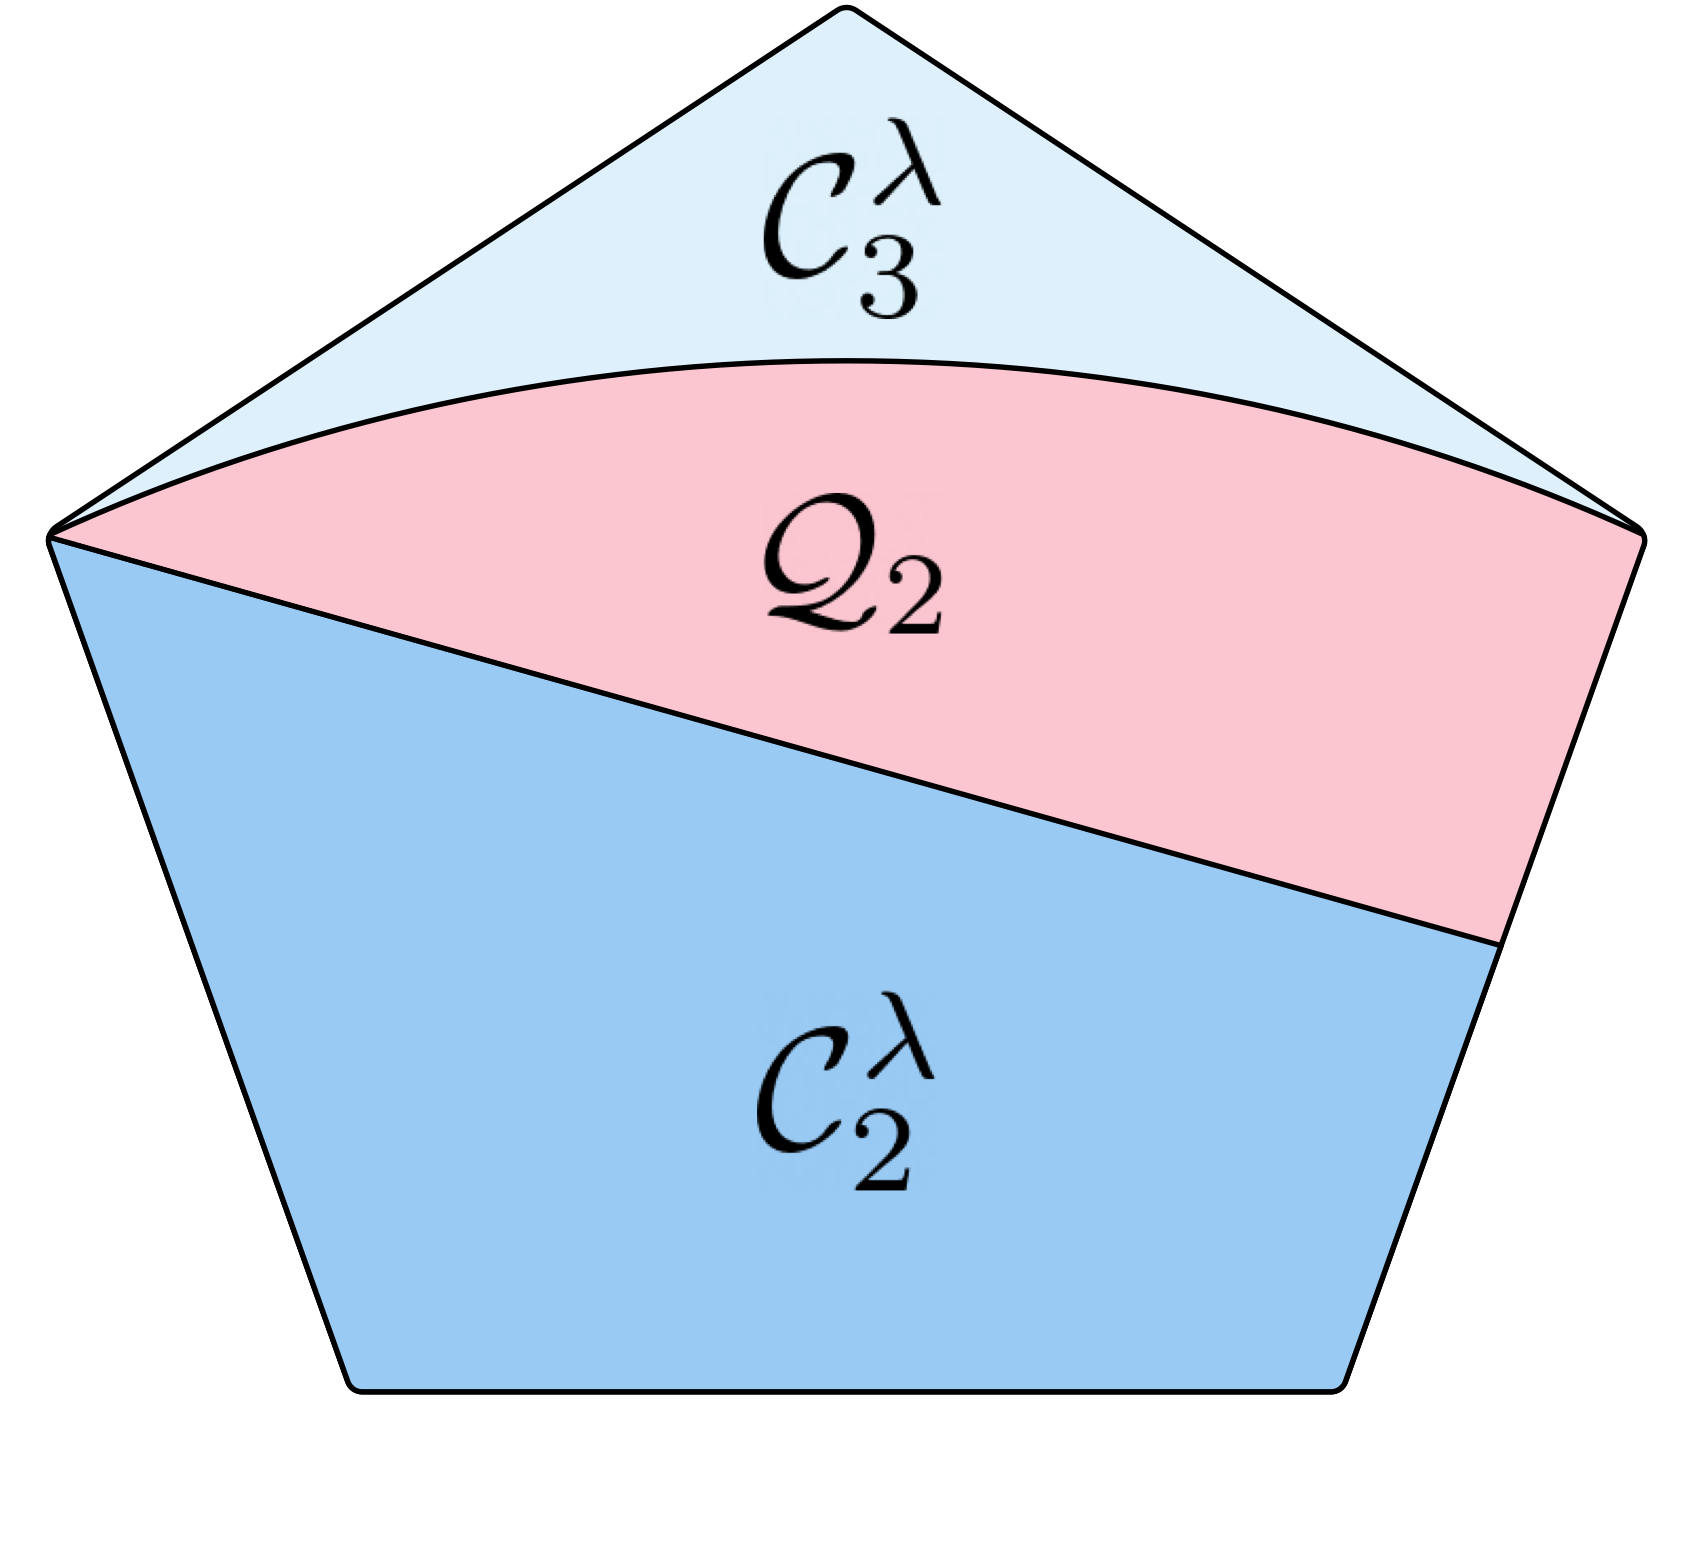
\includegraphics[width=.8\columnwidth]{behaviors.png}
			 	\end{minipage}
			 	%
				\begin{minipage}[c]{0.55\textwidth}
					\caption{Pictorial representation of prepare and measure behaviors. $\mathcal{C}_2^\lambda$, arising from $2$-dimensional classical communication with shared randomness, is a subset of any $\mathcal{C}_d^\lambda$ with $d > 2$ (eq.~\ref{eq:pam-classical-sr}). Qubit preparations, $\mathcal{Q}_2$, can behave in ways that violate the facets of $\mathcal{C}_2^\lambda$ \cite{gallego_pam_2010}.}	
            		\label{fig:pam-behaviors}
			    \end{minipage}
			    %
			\end{figure}
			            
            \ornamentbreak
            
            In recent years, a multitude of dimension and nonclassicality witnesses for prepare and measure scenarios have been proposed \cite{gallego_pam_2010,brunner_dimension_2013,sikora_dimension_2016,dallarno_robustness_2012,de_vicente_bound_2019,bowles_certifying_2014,wehner_lower_2008} and some of them experimentally tested \cite{hendrych_experimental_2012,ahrens_experimental_2012,dambrosio_highdimensional_2014}. More stringent conditions can also be used to perform self-testing of states and measurements, which can be used to certify the use of mutually unbiased bases, nonprojective measurements, or targeted sets of states \cite{tavakoli_selftesting_2018,farkas_selftesting_2019,wei_selftesting_2019,mironowicz_fouroutcome_2019,tavakoli_selftesting_2020,miklin_universal_2021,moreno_pamdense_2021}. All the while, known computational methods can aid in bounding the set of finite dimensional quantum correlations in prepare and measure scenarios \cite{navascues_bounding_2015,navascues_characterizing_2015}. The prepare and measure scenario and its sequential, or prepare-transform-and-measure, variations \cite{mohan_sequential_2019,miklin_sequentialunsharp_2020}, are also expected to serve as building blocks for quantum networks \cite{bowles_pamnetworks_2015,wang_pamnetworks_2019}. Complementing their versatility, they can also be seen as a physical implementation of many paradigmatic communication protocols such as random access coding and dense coding, which I now briefly introduce.


    %%%%%%%%%%%%%%%%%%%%%%%%%%%%%%%%%%%%%%%%%%%%%%
    \section{Prepare and measure communication protocols}
    \label{sec:communication-protocols}

        The preeminent practical interest in prepare and measure scenarios is due to the fact that quantum communication can beat classical protocols in many tasks that can me modeled as preparing and measuring states. These include cryptographic key distribution \cite{pawlowski_pamqkd_2011}, secret sharing \cite{schmid_secret_2005} and communication complexity scenarios \cite{buhrman_communicationreview_2010}. Simplifiedly, the latter deals with the question of how much is the least amount of communication needed to compute or approximate some function $f(x,y)$ when the inputs $x$ and $y$ are distributed among distant parties. Prepare and measure scenarios clearly resemble this structure. To close the gap, all we have to do is to stipulate a figure of merit that, generally depending on $f$, measures how well the protocol at hand performs. If we additionally manage to show some separation between the best performance achievable, for instance, in $\mathcal{C}_d^\lambda$ against $\mathcal{Q}_d$, we can prove quantum advantage in the task. A special and widely studied choice of $f(x,y) = x_y$ leads us to the so-called \emph{random access coding} (RAC) protocol.

        \subsection{Random access coding}
        \label{sec:racs}

            An $\rac{n}{d}{m}$ random access code (RAC) is a communication task in which a party --- commonly Alice --- is given a $n$-length $d$itstring $\mathbf{x} = x_1 x_2 \ldots x_n$, with each $x_i \in \{0, \ldots, d - 1 \}$, and required to encode it in another ditstring $\mathbf{a}$ of length $m$, where $m < n$. Her encoded message is then sent to Bob, who is queried with an $y \in \{1, \ldots, n\}$ representing which dit of the original message $\mathbf{x}$ he must guess. In each round of a RAC, Bob's probability of guessing the right value is given by $p(b = x_y \mid \mathbf{x}, y)$, and this is the quantity we seek to maximize. A RAC can thus be seen as a (potentially lossy) information compression protocol where Alice and Bob must cooperate to perform as best as possible. Their performance is typically measured through the \emph{worst-case success probability} $p_{\text{worst}}$, defined as the minimum guess probability $p(b = x_y \mid \mathbf{x}, y)$ occurring for their particular encoding-decoding strategy. When the best possible strategy for an $\rac{n}{d}{m}$ scenario is such that $p_{\text{worst}} \leq 1/d$, the RAC is said to not exist, as in that case a better or equivalent performance could be achieved through independently guessing.

			Such a task may be physically implemented in various ways. Among the simplest are the \emph{deterministic strategies}. In it, Alice must encode $\mathbf{x}$ into the $m$-dits message $\mathbf{a} = \mathcal{E}(\mathbf{x})$, where $\mathcal{E} : \{0, \ldots, d - 1\}^n \mapsto \{0, \ldots, d - 1\}^m$ is an encoder function. Given $\mathbf{a}$ and a $y$, Bob employs one out of $n$ decoding functions $\mathcal{D}_y : \{0, \ldots, d - 1\}^m \mapsto \{0, \ldots, d - 1\}$ to generate his answer. The probability of Bob answering $b$ is thence given by $\condprob{b}{\mathbf{x}, y} = \delta\left[b, (\mathcal{D}_{y} \circ \mathcal{E})(\mathbf{x})\right]$. In the simplest $\rac{2}{2}{1}$ RAC, deterministic strategies lead to a $p_{\text{worst}} = 0$, and probabilistic (but still uncorrelated) strategies render a $p_{\text{worst}} = 0.5$ \cite{ambainis_qracsoriginal_1999,ambainis_srqracs_2009}. Interestingly, shared randomness (SR) is known to drastically improve the performance in this task. By sharing randomness, Alice and Bob may cooperate via predetermined classical strategies. Effectively, the encoding and decoding functions become correlated through the shared variable $\lambda$, and we end up with probability distributions over deterministic strategies. In this case, it is known that an SR-RAC's worst case success probability is effectively lifted to the deterministic RAC \emph{average} success probability $\psuc$ \cite{ambainis_srqracs_2009}, i.e., 
            \begin{equation}
                p_{\text{worst}}^{\text{SR}} = p_{\text{avg}} \equiv \frac{1}{nd^n} \sum_{\mathbf{x},y} \condprob{b=x_y}{\mathbf{x},y} .
                \label{eq:rac-p-avg}
            \end{equation}
            %
			Ibidem, it is also argued that an optimal deterministic strategy in $\rac{n}{2}{1}$ RACs is reached through majority encoding with identity decoding. In our $\rac{2}{2}{1}$ case, this translates to Alice mapping $(00, 01, 10, 11) \mapsto (0, c, c, 1)$, where $c$ stands for any choice, and Bob outputting exactly what he gets. As this achieves a $p_{\text{avg}} = 0.75$, it follows from eq.~\ref{eq:rac-p-avg} that it is possible to reach $p_{\text{worst}} = 0.75$ by exploiting shared randomness.
			

			% For a concrete example, consider the simplest $\rac{2}{2}{1}$ scenario. When no SR is allowed, $p_{\text{worst}} \leq 0.5$ . With SR, however, Alice and Bob can cooperate in the following way. Before each round, a random variable $\lambda \in \{0, 1\}$ instructs Alice to send $\mathbf{a} = x_\lambda$. Bob knows $\lambda$, so if he's queried with $y = \lambda$, he can answer correctly with certainty; otherwise he can just flip a coin. Of course, we still have $p_{\text{worst}} \leq 0.5$ in this situation. However, it is known from \cite{ambainis_srqracs_2009} that when SR is allowed, the best possible strategy is such that \review{Confirmar se é isso mesmo}
            % %
            % \begin{equation}
            %     p_{\text{worst}} = p_{\text{avg}} \equiv \frac{1}{nd^n} \sum_{\mathbf{x},y} \condprob{b=x_y}{\mathbf{x},y} ,
            %     \label{eq:rac-p-avg}
            % \end{equation}
            % %
            % for an uniform distribution on $y$, therefore proving that a $\rac{2}{2}{1}$ SR-RAC with $p_{\text{worst}} = 0.75$ exists.

            Something else that can further improve performance is allowing for quantum communication. In this case, we interpret the encoders $\mathcal{E}(\mathbf{x}) = \rho_x \in \mathcal{D}(d)$ as preparation procedures and the decoders $\mathcal{D}_y = \{ E_{b \mid y} \}_b$ as quantum measurements. These so-called \emph{quantum random access codes} (QRACs) first appeared in \cite{wiesner1983conjugate} and were later rediscovered and linked to quantum automata in \cite{ambainis_qracsoriginal_1999}. With this popularization, multiple new results and experimental demonstrations regarding the existence and advantage of QRACs over their classical counterparts rapidly ensued \cite{nayak1999optimal,ambainis2002dense,hayashi_41qracs_2006,ambainis_srqracs_2009,spekkens2009preparation,pawlowski_pamqkd_2011}. QRACs can largely outperform shared randomness strategies in the $\rac{2}{2}{1}$ RAC, getting up to $p_{\text{avg}} \approx 0.853553$.

            Random access codes can be interpreted as specific instances of prepare and measure scenarios or, conversely, the latter can be seen as physical implementations of RACs. Mapping QRACs to PM scenarios with quantum communication, for instance, amounts to choosing $\abs{\mathcal{X}} = d^n$ preparations $\rho_{x} \in \mathcal{D}(d)$, and $\abs{\mathcal{Y}} = n$  choices of POVMs with $\abs{\mathcal{B}} = d$ outcomes each \cite{de_vicente_bound_2019}. The set of behaviors is then $\mathcal{Q}_{d,d,d^n,n}$, and optimizing the protocol means looking for a $\mathbf{p} \in \mathcal{Q}_{d,d,d^n,n}$ that maximizes either $p_{\text{worst}}$ or $p_{\text{avg}}$, depending on which is the chosen figure of merit. In the next chapter we will make use of this mapping to demonstrate an interesting quantum advantage activation phenomenon in QRACs.

            Additionally to RACs, SR-RACs and QRACs, one could also investigate SR-QRACs \cite{ambainis_srqracs_2009}, EA-RACs \cite{pawlowski_earacs_2010} and EA-QRACs, where ``EA'' stands for ``entanglement-assisted''. Each of these cases (which I will herein collectively refer to as simply ``RACs'') could analogously be mapped to a PM scenario, and the optimal solutions would be searched for inside the PM behavior sets $\mathcal{C}$, $\mathcal{C}^\lambda$, $\mathcal{Q}$, $\mathcal{Q}^\lambda$, $\mathcal{C}^\rho$ and $\mathcal{Q}^\rho$, respectively, all with subscripts $d,d,d^n,n$.

            To end this section, I note that while RACs can be cast as an instance of prepare and measure, the inverse is not true. Investigating what different kinds of \emph{information retrieval tasks} \cite{emeriau_torpedo_2020} arise from such other instances could be an interesting research problem.

        %%%%%%%%%%%%%%%%%%%%%%%%%%%%%%%%%%%
        \subsection{Dense coding}
        \label{sec:dense-coding}

            Holevo's bound guarantees that $n$ qubits can perfectly encode no more than $n$ bits of information \cite{holevo-bound-1973}. Calling to mind that $n$ qubits require $2^n - 1$ complex coefficients to be fully described, this result comes to be tremendously surprising. Looking more closely, the setting where this conclusion arises from is a prepare and measure scenario with quantum communication but independent devices. Another seminal result, named \emph{dense coding}, proves that when the devices are not independent, but rather, share a maximally entangled state as a resource, it becomes possible to communicate two bits by sending a single qubit.

            Dense coding was first proposed by Bennett and Wiesner \cite{bennett_1992_superdense} similarly to the following argument. Let Alice and Bob share a two-qubit maximally entangled state $\ket{\Phi^+} = \frac{1}{\sqrt{2}} \sum_{i = 0}^{1} \ket{ii}$ (the same argument is valid for any unitary transformation of it). Her task is to communicate one out of four messages to Bob. We label those messages with choices from the ordered set $\mathcal{X} = (0, 1, 2, 3)$, which could be perfectly encoded with two bits. Alice and Bob, prior to the experiment, agree on some special set of transformations, hereby $\Lambda = (\id,\sigma_x, \sigma_y, \sigma_z)$ --- where $\sigma_i$ are the Pauli matrices ---, to represent the respective encodings. Alice's encoding of $x$ is a simple matter of applying $\Lambda_x$ to her share of $\ket{\Phi^+}$. After receiving her qubit, Bob will thus have the state $\left( \Lambda_x \otimes \id \right) \ketbra{\Phi^+}{\Phi^+}$. The four possibilities are mutually orthogonal, hence can be perfectly distinguished by some suitable measurement (e.g., a standard Bell-basis measurement). Therefore, Bob will be able to perfectly recover $x$ even with a single qubit of communication.
            
            Purposefully, I have framed the protocol in the previously introduced notation for a prepare and measure scenario with quantum communication and entanglement assistance. My intention was to suggest that dense coding can be implemented as a special instance of prepare and measure scenarios. In chap. \ref{chap:pam-quantum}, we will see how it indeed can. More than that, several generalizations of this protocol are possible. The most straightforward ones are to allow for higher dimensional communication and entanglement \cite{bennett_1992_superdense} or mixed-state entanglement \cite{barenco_dense_1995}. Recently, discussions have also been opened in regard to unbounded entanglement \cite{tavakoli_eapam_2021} or even dense coding protocols with errors \cite{nayak_rigidity_2020,moreno_pamdense_2021}. Chapter \ref{chap:pam-quantum} will also detailedly discuss how we can use insights from prepare and measure scenarios to prove interesting results for the latter case.